\makeatletter
\def\input@path{{../}}
\makeatother

\documentclass[/main.tex]{subfiles}
\graphicspath{{./pics/}{appPeakShape/pics/}}
\begin{document}

\onlyinsubfile{\appendix}
\chapter{Peak Shape Description and Measurement} \label{app:peakshape}

\section{Peak Shape Function and Parameters}
A moneenergetic energy peak in the \MJD\ is typically modelled using the following peakshape function
\begin{equation} \label{eq:peakshape}
  \begin{aligned}
    \mathrm{PS}(E; A, \mu, \sigma, f_{tail}, \tau, h_{step}) &= A\big((1-f_{tail})\mathrm{Gaus}(E; \mu, \sigma) \\&+ f_{tail}\cdot\mathrm{ExGaus}(E; \mu, \sigma, \tau) \\&+ \frac{h_{step}}{2}\mathrm{erfc}(\frac{E-\mu}{\sqrt{2}\sigma})\big)
  \end{aligned}
\end{equation}
where $A$ is the total area of the peak.
The peak shape consists of a Gaussian component:
\begin{equation}
  \mathrm{Gaus}(E; \mu, \sigma) = \frac{1}{\sqrt{2\pi\sigma^2}}\mathrm{exp}(-\frac{(E-\mu)^2}{2\sigma^2})
\end{equation}
and a low energy (LE) tail, defined as an exponentially modified Gaussian (exGaus) component:
\begin{equation}
  \mathrm{ExGaus}(E; \mu, \sigma, \tau) = \frac{1}{2|\tau|} \mathrm{erfc}(\mathrm{sgn}(\tau)\frac{(E-\mu) + \frac{\sigma^2}{\tau}}{\sqrt{2}\sigma})\mathrm{exp}(\frac{E-\mu}{\tau}+\frac{\sigma^2}{\tau^2})
\end{equation}
$\sigma$ represents the gaussian width, $\tau$ represents the length of the LE tail, and $f_{tail}$ represents the fraction of the peak contained in the LE tail.
Note that this formulation of the ExGaus function allows for negative values of $\tau$, resulting in a high energy tail instead of a low energy tail.
These three parameters combine to define the width of the peak, while $\mu$ represents the mean of the Gaussian component; note that the mean of the peak as a whole will be lower due to the LE tail.
The LE tail originates from position dependant factors in the detectors that cause energy loss, including charge trapping and transition layers.
Finally, the peak shape contains a step component, described by the complementary error function (erfc), where $h_{step}$ defines the fraction of the peak amplitude that appears in the step.
The step is caused by factors that cause enough energy loss to pull events entirely out of the peak, such as low angle scattering of a $\gamma$ before entering a detector and detector transition layers.
Events in the step component are not considered part of the full energy peak, and the step is primarily a factor for calibration events which must pass through the copper cryostat which is not true of events that originate in the detectors.
For this reason, the step is not considered when optimizing the signal ROI.
\begin{figure}
  \centering
  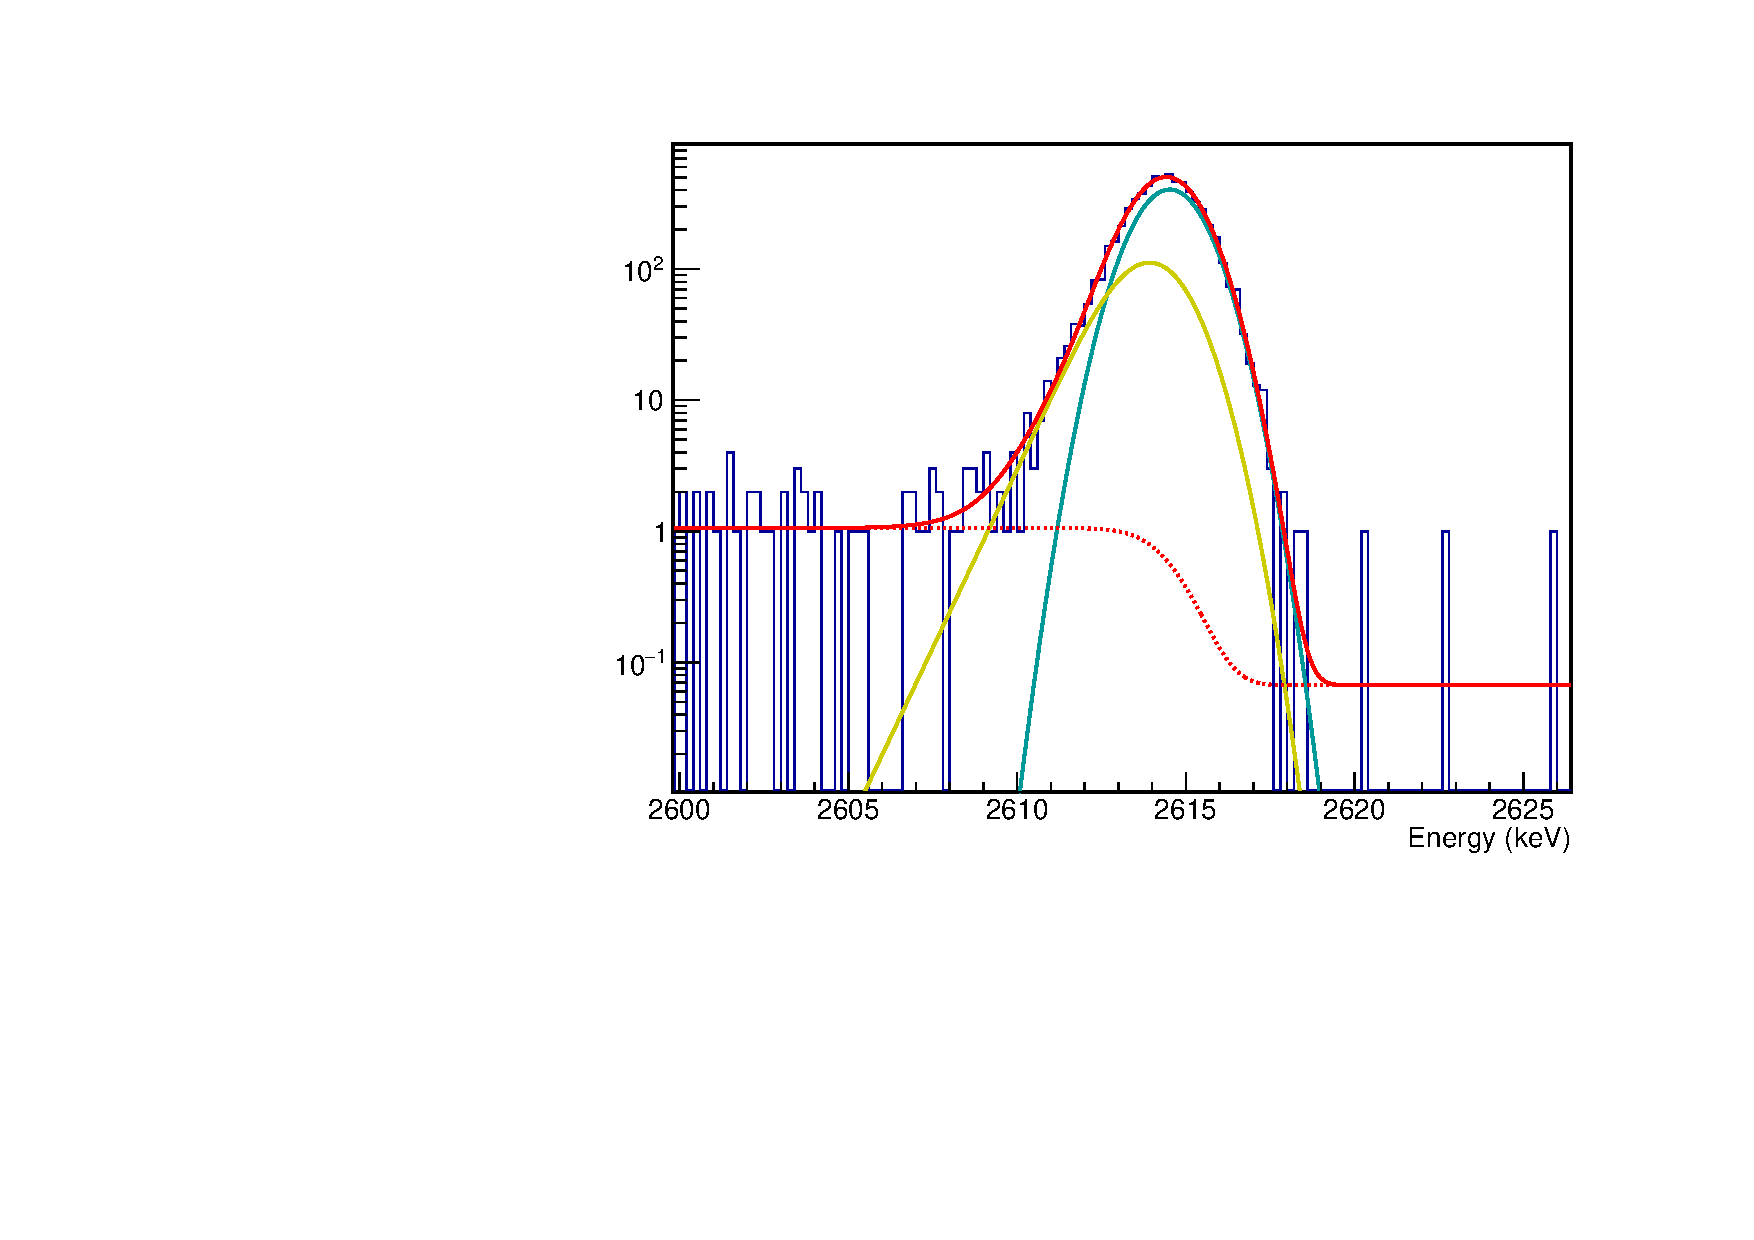
\includegraphics[width=0.8\textwidth]{peakshape}
  \caption[Peak shape function]{\label{fig:peakshape}
    A 2614~keV calibration peak fitted to the peakshape function described by equation~\ref{eq:peakshape}. The Gaussian component is shown in teal, the low energy tail in gold, the step in dashed red, and the combined peak shape in red.
  }
\end{figure}
The peak shape function is shown in Figure~\ref{fig:peakshape}.
\\
This peak shape function can be optionally extended with the addition of a high energy tail as follows:
\begin{equation}
  \begin{aligned}
    \mathrm{PS}(E; A, \mu, \sigma, f_{LT}, \tau_{LT}, f_{HT}, \tau_{HT}, h_{step}) &= A\big((1-f_{LT}-f_{HT})\mathrm{Gaus}(E; \mu, \sigma) \\&+ f_{LT}\cdot\mathrm{ExGaus}(E; \mu, \sigma, \tau_{LT}) \\&+ f_{HT}\cdot\mathrm{ExGaus}(E; \mu, \sigma, -\tau_{HT}) \\&+ \frac{h_{step}}{2}\mathrm{erfc}(\frac{E-\mu}{\sqrt{2}\sigma})\big)
  \end{aligned}
\end{equation}
Typically, no high energy tail is used, meaning $f_{HT}=0$.
A high energy tail is necessary only if an abnormal peakshape appears.
This can occur if the energy filter parameters are mis-set, or if peaks other than full energy $\gamma$ peaks are being fit, as is the case in Section~\ref{sec:Co56}, where the single- and double-escape peaks are used.
\\
A simultaneous fit of many peaks in a calibration spectrum is performed in order to define the peak shape parameters at all energies.
The peak shape parameters are defined as independant functions of energies and several hyperparameters as follows
\begin{itemize}
\item $A$ is independant of energy, since it depends on the relative intensities and the different detection efficiencies of each $\gamma$.
\item $\mu$ is also independant of energy.
  $\mu$ is ostensibly linear with respect to energy; however, due to local and global energy nonlinearities, in order to avoid systematic errors in the other peak shape parameters, this parameter is treated as independant.
\item $\sigma$ is defined as follows
  \begin{equation}
    \sigma(E) = \sqrt{\sigma_0^2 + \sigma_1^2E + \sigma_2^2E^2}
  \end{equation}
  $\sigma_0$ arises primarily from electronic noise. $\sigma_1$ arises primarily from the Fano factor $F$, and is ostensibly
  \begin{equation}
    \sigma_1^2 = (2.35)^2F\epsilon E
  \end{equation}
  where $F=0.08$ and $\epsilon=2.96$~eV is the electron-hole production energy.
  In actuality, other factors also contribute to $\sigma_1$, so it is measured to be larger than expected.
  $\sigma_2$ arises from a variety of systematic energy uncertainties, including charge trapping, gain drift and small errors in energy calculation.
\item $f_{tail}$ is defined to be constant with respect to energy.
\item $\tau$ is defined as linear with respect to energy
  \begin{equation}
    \tau(E) = \tau_0 + \tau_1
  \end{equation}
  $\tau_1$ arises primarily from charge trapping and transition layer events, each of which cause charge loss.
  $\tau_0$, while expected to be zero, is necessary in order to obtain a strong fit result.
\item $h_{step}$ is defined as
  \begin{equation}
    h_{step}(E) = \frac{h_0}{E^2} + h_1E^{-0.88}
  \end{equation}
  The inverse square term arises from low angle scattering of $\gamma$s as they approach the detector.
  The second power law term arises from transition layer events, and the power of -0.88 was empirically measured in simulations and data.
  This model is described in greater detail in Section~\ref{sec:stepheight}.
\end{itemize}
The fit result of a simultaneous fit of 18 peaks from a 6~hour long \Th{228} calibration run is shown in Figure~\ref{fig:simultaneousfit}.
\begin{figure}[p]
  \centering
  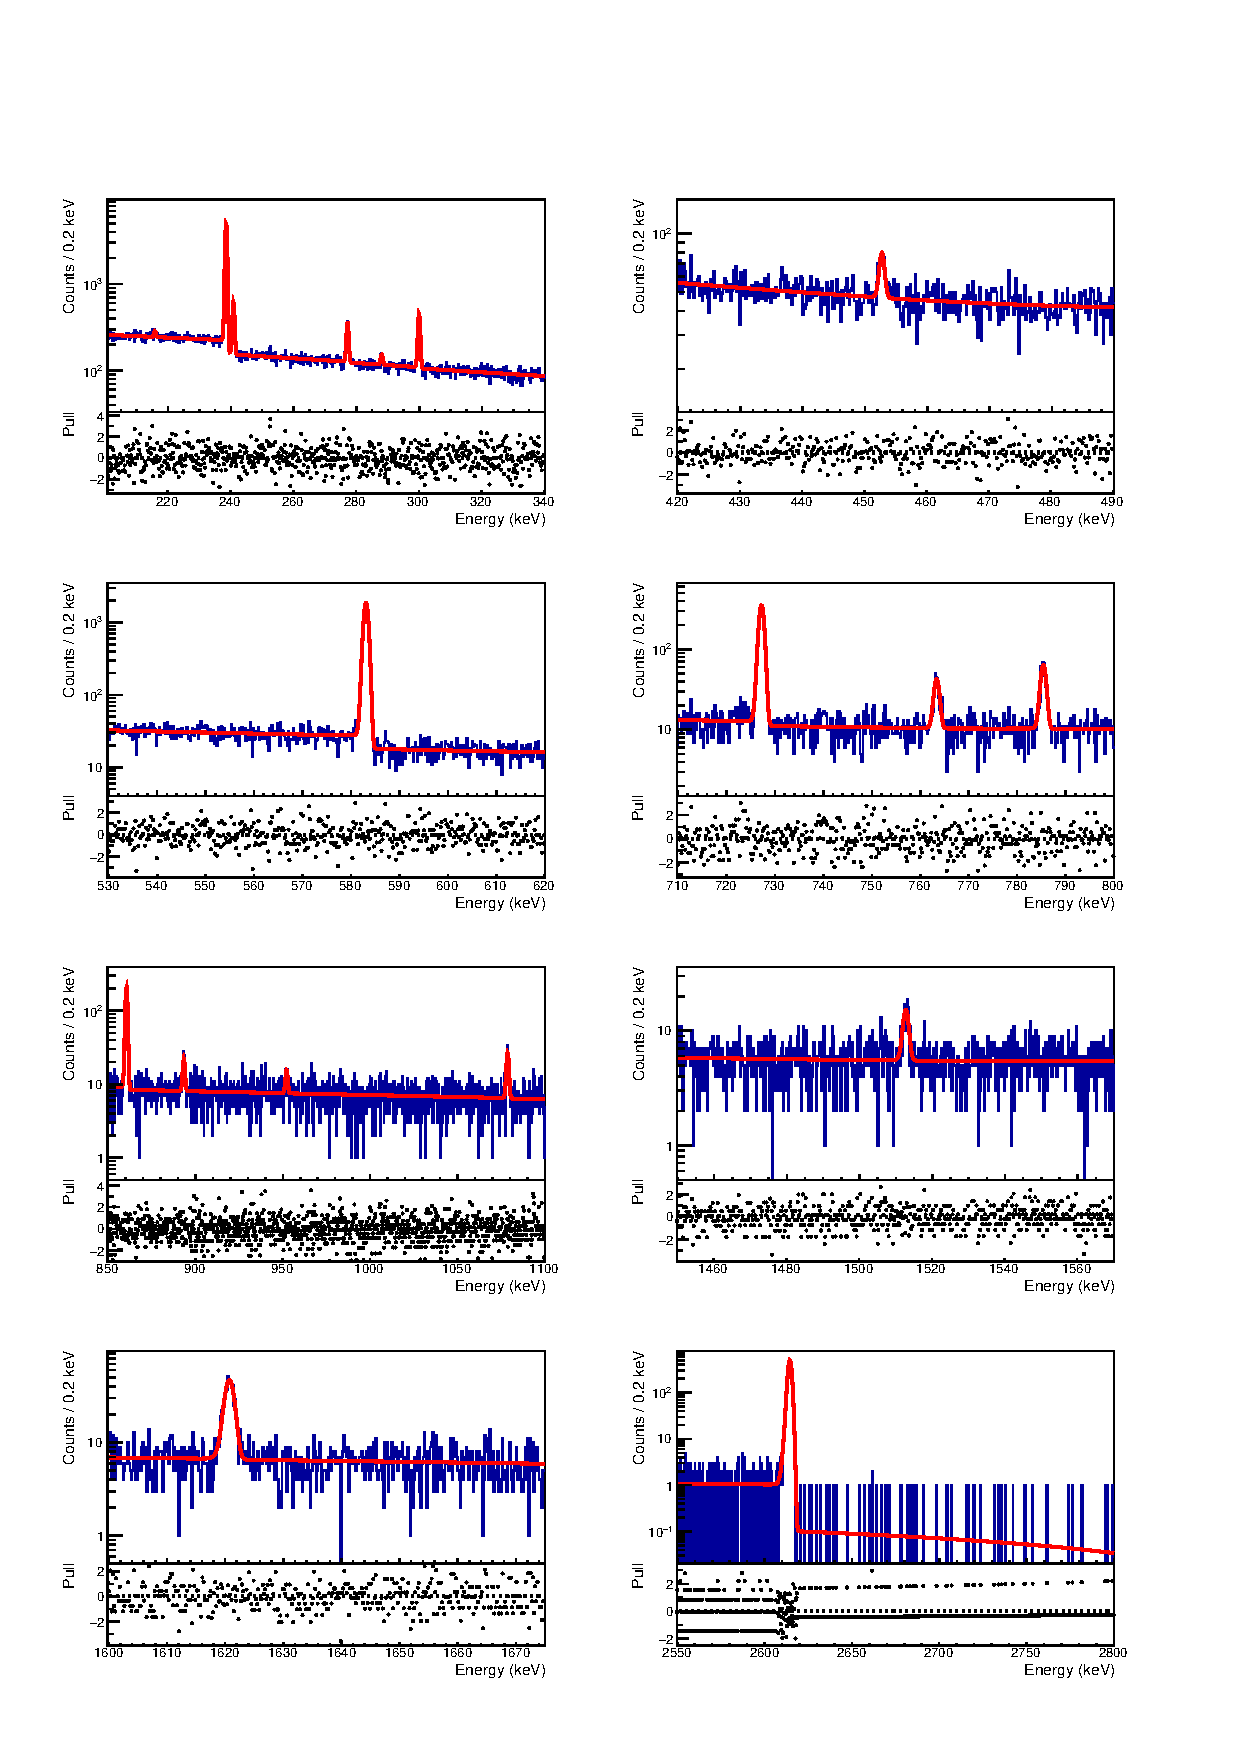
\includegraphics[width=0.8\textwidth]{fitResults}
  \caption[Simultaneous peak fit of \Th{228} calibration]{\label{fig:simultaneousfit}
    A simultaneous fit of 18 peaks from a 6~hour long \Th{228} calibration run)
  }
\end{figure}
\section{Performing a Simultaneous Fit} \label{sec:fitter}
Because of the large number of fit parameters (${\sim}35$~parameters are used for weekly calibrations and ${\sim}100$~parameters are used with high statistics calibrations to perform more detailed characterizations of parameters), and because of the highly correlated nature of some of the parameters, the fit result is heavily dependant on the initial parameter guess.
To ensure convergence on the global minimum of the negative log-likelihood in a timely manner, Hamiltonian Monte Carlo (HMC) is used\cite{DUANE1987}\cite{2012Neal}.
HMC is a Markov Chain Monte Carlo (MCMC) technique that uses the parameter gradient of the negative log-likelihood in order to take large steps through the parameter space with a high acceptance rate.
Several adaptations to the step sizes are applied, which prevent the algorithm used from exactly converging to the posterior described by the log-likelihood with a flat prior.
First, the step size is increased by a factor of 1.1 after each successful step and decreased by a factor of 1.2 after each unsuccessful step.
This adaptation asymptotically results in an acceptance rate of ${\sim}2/3$, a target suggested by \cite{2012Neal}.
Second, the mass scale matrix is adapted to equal the diagonal elements of the Fisher information metric between each step.
This adaptation is based on Riemann Manifold HMC\cite{Girolami2011}, although it does not properly evolve the metric between steps and will therefore fail to converge exactly.
The combination of these adaptations results in a quick and reliable convergence that approximates the posterior, and is very useful as a burn-in when fitting.
The adaptations above are combined are run over 200~HMC steps, using the leapfrog algorithm with 50 leapfrog steps for each HMC step.
In addition, the evaluation of the parameter gradient of the negative log-likelihood is performed analytically, which helps to speed up evaluation and ensure reliability.
\\
After this HMC burn in is performed, the minimum negative log-likelihood sample is used as an initial parameter guess for a gradient descent fit.
The Minuit fitting package is used to perform this fit\cite{minuit}.
Minuit evaluates for the parameters that maximize the likelihood and uses the Hessian matrix to obtain a covariance matrix.
This result is used to obtain the values and errors of the calibration parameters.
\\
\section{Computing Auxiliary Parameters}
In addition to the bare parameters used to describe this peakshape model, other auxiliary parameters are often useful to calculate when using this model to characterize detectors.
Examples of such parameters include the values of the individual peakshape parameters for an arbitrary peak energy, and other parameters that can be derived from the peakshape function such as the peak centroid or full width at half max (FWHM).
The peak centroid is used for the first stage of calibration and the FWHM is used when optimizing the ROI for a peak.
It is not ideal to numerically compute these parameters directly from the data, because such a measurement would be biased by the background or by the step component of the peakshape, which is not intrisic to the detectors.
To do this, first we calculate the value of the detector-intrisic peak shape parameters (i.e. $\mu$, $\sigma$, $f_{LE}$, $\tau_{LE}$, $f_{HE}$ and $\tau_{HE}$ at the desired energy using the functions used to describe each parameter.
From here, derived parameters can be calculated; for example, the centroid is
\begin{equation}
  \mathrm{cen}(\mu, \sigma, f_{LE}, \tau_{LE}, f_{HE}, \tau_{HE})=\mu - f_{LE}\cdot\tau_{LE} + f_{HE}\cdot\tau_{HE}
\end{equation}
and the FWHM is numerically calculated by finding the half max energies and taking the difference between them, assuming no background and no step.
The uncertainties on these parameters is computed from the covariance matrix.
For parameter $\theta$:
\begin{equation}
  \sigma_\theta^2= \sum_{i=0}^{N}\sum_{j=0}^{N} \frac{\partial\theta}{\partial p_i} \Sigma_{i,j} \frac{\partial\theta}{\partial p_j}
\end{equation}
where $p_i$ are the set of model parameters.
\\
\section{The Step Height Model} \label{sec:stepheight}
The dependancy of the step height on energy is described by
\begin{equation}
  h_{step}(E) = \frac{h_0}{E^2} + h_1E^{-h_2}
\end{equation}
The inverse square component arises from low angle scattering of $\gamma$s as they approach the detectors.
This inverse square dependence can be analytically derived by taking the Compton scattering differential cross section in the limit as scattering angle approaches 0\cite{2011Oberer}.
$h_0$ increases linearly with the thickness of shielding between the source and the detector.
As a result, the model parameters measured are valid only for $\gamma$s from the calibration source; peaks generated by other sources may have different steps, and peaks generated from a source internal to the detector would be expected to measure $h_0=0$.
\\
The second power law term arises from the transition layer of the detectors.
Because of this model is nonlinear, floating the power parameter results in unreliable fitting for the standard 90-minute calibration runs, so $h_2$ is empirically measured using both data and simulations to be -0.88.
Many simulations of the \Th{228} calibration source were run using the dead layer model described in equation~\ref{eq:dlmodel}, and the thickness of the transition layer varied between 0~and 2~mm.
For each simulation, a simultaneous fit of many peaks was performed, floating all of the step height parameters.
The values of $h_2$ measured are shown in Figure~\ref{fig:stepheightpars_sim}, and have a stable value of -0.88 for dead layer thickness of $<1$~mm.
Typical dead layer thicknesses for detectors are ${\sim}0.5$~mm.
\begin{figure}[t]
  \centering
  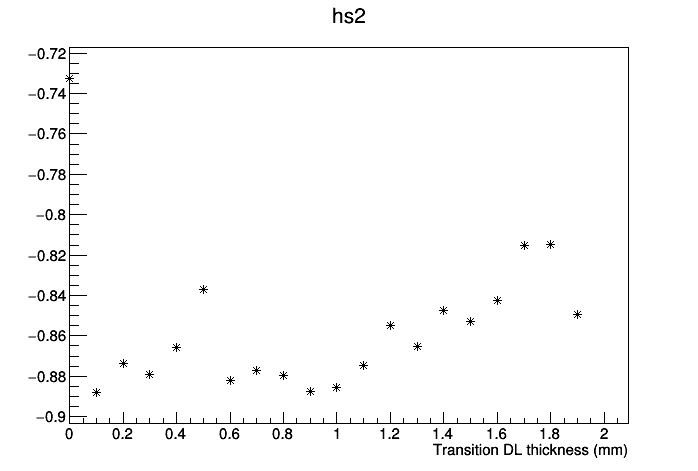
\includegraphics[width=0.8\textwidth]{hs2_tl}
  \caption[Simulated dependance of $h_2$ on transition layer thickness] {\label{fig:stepheightpars_sim}
    Values of $h_2$ from the step height model measured using a simultaneous peak fit for simulations of the \Th{228} calibration source using different transition layer thicknesses.
  }
\end{figure}
To measure this parameter from data, many peaks in a long calibration run were used.
A fit was then performed for each detector, floating $h_2$ and fixing $h_{0}$.
The value of $h_0$ is fixed to a value extracted from a fit of a calibration simulation that does not include the dead layer.
The values of $h_2$ were measured from simultaneous fits of the spectrum measured for each detector in a long calibration run, and are shown in Figure~\ref{fig:stepheightpars_dat}.
The measured values have large systematic uncertainties that are not accounted for in the fits, but the mean is consistent with the value of -0.88 measured using the simulations.
\begin{figure}[t]
  \centering
  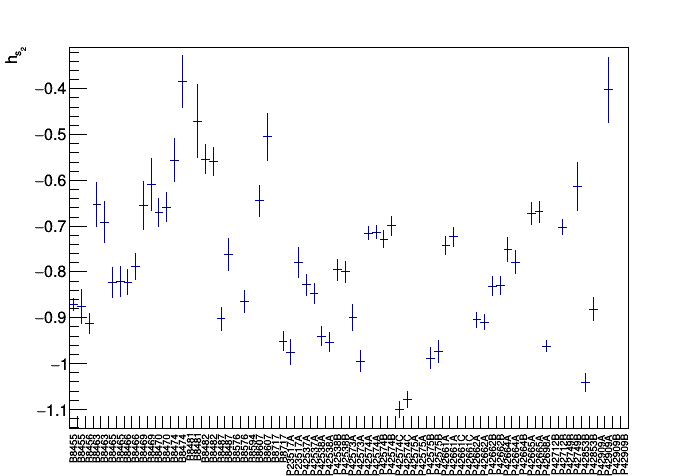
\includegraphics[width=\textwidth]{hs2}
  \caption[Measured values of $h_2$ in calibration data] {\label{fig:stepheightpars_dat}
    Values of $h_2$ from the step height model measured using a simultaneous peak fit of the measured \Th{228} calibration spectrum. $h_0$ was fixed to values measured from simulations.
  }
\end{figure}


\section{GAT Implementation}
Implementations of the peak shape function, the parameter gradient of the peak shape function, the CDF of the peak shape function, and functions calculating various auxillary parameters such as the FWHM, centroid and standard deviation are included in \texttt{GATPeakShapeUtil.hh}.
Implementation of an energy range with a single peak on top of a quadratic background, along with tools for fitting this energy region are included in \texttt{GATPeakShape.hh}.
Implementation of an energy region with multiple peaks included, with the peakshape parameters determined by functions of energy and various hyperparameters are included in \texttt{GATMultiPeakRegion.hh}.
Implementation of the multi peak fitter, which manages many \texttt{GATMultiPeakRegion}s and the various parameter functions and hyperparameters, as well as many tools for computing auxiliary parameters at various energies, are included in \texttt{GATMultiPeakFitter.hh}.
Implementation of a combined likelihood function to be used for simultaneous fitting is included in \texttt{GATGlobalFitFCN.hh}.
Implementation of the HMC algorithm described in Section~\ref{sec:fitter} is contained in \texttt{GATHybridMonteCarlo.hh}.
\\

\onlyinsubfile{
  \bibliographystyle{plain}
  \bibliography{../main}
}

\end{document}